\documentclass{minimal}
\usepackage{graphicx,color}
\usepackage[papersize={576.00bp,432.00bp},text={576.00bp,432.00bp}]{geometry}
\begin{document}
\centering
% Title: gl2ps_renderer figure
% Creator: GL2PS 1.4.0, (C) 1999-2017 C. Geuzaine
% For: Octave
% CreationDate: Wed Aug 12 00:41:49 2020
\setlength{\unitlength}{1pt}
\begin{picture}(0,0)
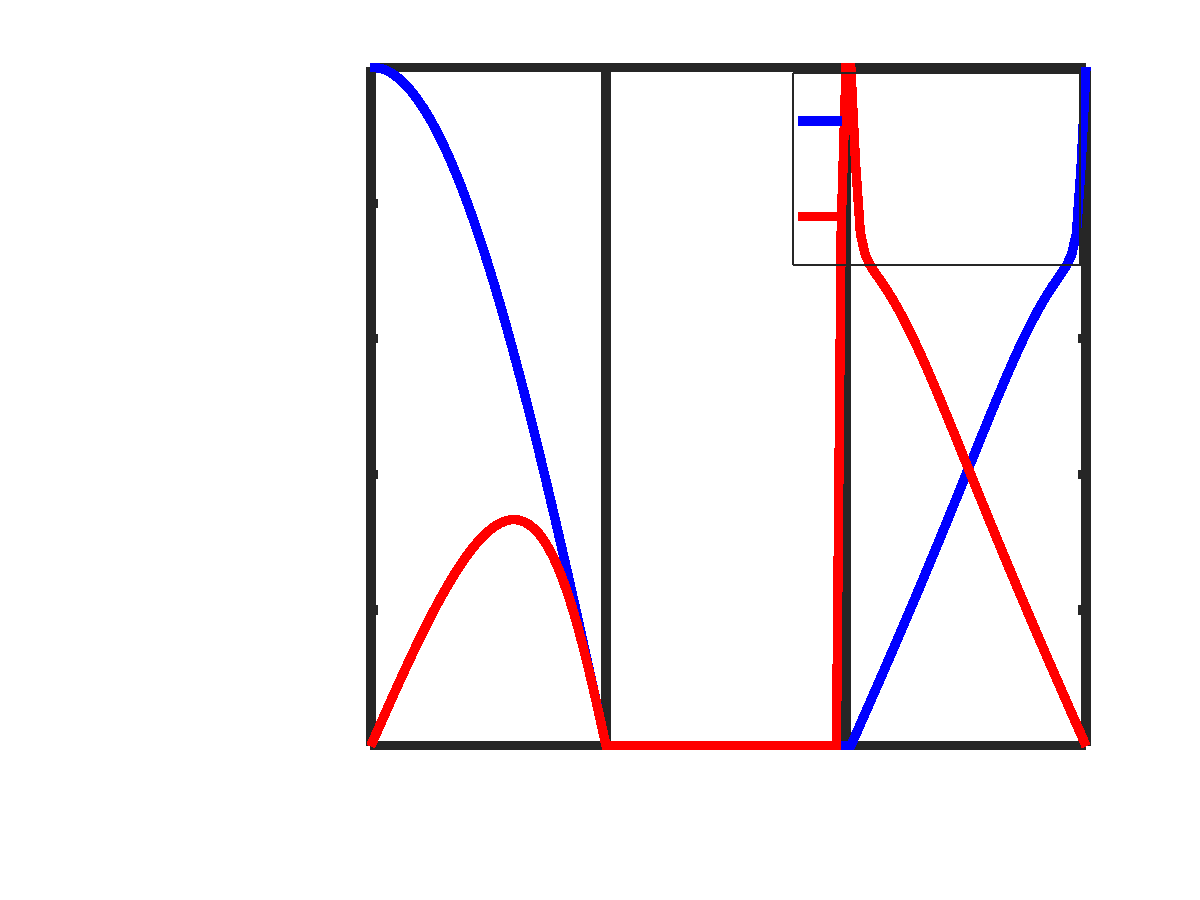
\includegraphics{m2hx0pt1hy0hz0-inc}
\end{picture}%
\begin{picture}(576,432)(0,0)
\fontsize{50}{0}
\selectfont\put(172.999,74.0076){\makebox(0,0)[r]{\textcolor[rgb]{0.15,0.15,0.15}{{0}}}}
\fontsize{50}{0}
\selectfont\put(172.999,139.126){\makebox(0,0)[r]{\textcolor[rgb]{0.15,0.15,0.15}{{0.02}}}}
\fontsize{50}{0}
\selectfont\put(172.999,204.245){\makebox(0,0)[r]{\textcolor[rgb]{0.15,0.15,0.15}{{0.04}}}}
\fontsize{50}{0}
\selectfont\put(172.999,269.363){\makebox(0,0)[r]{\textcolor[rgb]{0.15,0.15,0.15}{{0.06}}}}
\fontsize{50}{0}
\selectfont\put(172.999,334.482){\makebox(0,0)[r]{\textcolor[rgb]{0.15,0.15,0.15}{{0.08}}}}
\fontsize{50}{0}
\selectfont\put(172.999,399.6){\makebox(0,0)[r]{\textcolor[rgb]{0.15,0.15,0.15}{{0.1}}}}
\fontsize{50}{0}
\selectfont\put(68.9989,236.804){\rotatebox{90}{\makebox(0,0)[b]{\textcolor[rgb]{0.15,0.15,0.15}{{$Im(E)$}}}}}
\fontsize{40}{0}
\selectfont\put(178.003,41.4484){\makebox(0,0)[l]{\textcolor[rgb]{0,0,0}{{$\Gamma$}}}}
\fontsize{40}{0}
\selectfont\put(290.893,41.4484){\makebox(0,0)[l]{\textcolor[rgb]{0,0,0}{{$X$}}}}
\fontsize{40}{0}
\selectfont\put(406.086,41.4484){\makebox(0,0)[l]{\textcolor[rgb]{0,0,0}{{$M$}}}}
\fontsize{40}{0}
\selectfont\put(521.28,41.4484){\makebox(0,0)[l]{\textcolor[rgb]{0,0,0}{{$\Gamma$}}}}
\fontsize{20}{0}
\selectfont\put(429.125,171.685){\makebox(0,0)[l]{\textcolor[rgb]{0,0,0}{{$h_x=0.1$}}}}
\fontsize{20}{0}
\selectfont\put(429.125,139.126){\makebox(0,0)[l]{\textcolor[rgb]{0,0,0}{{$h_y=0$}}}}
\fontsize{20}{0}
\selectfont\put(429.125,106.567){\makebox(0,0)[l]{\textcolor[rgb]{0,0,0}{{$h_z=0$}}}}
\fontsize{30}{0}
\selectfont\put(406.76,373.881){\makebox(0,0)[l]{\textcolor[rgb]{0,0,0}{{$m=2$}}}}
\fontsize{30}{0}
\selectfont\put(406.76,327.935){\makebox(0,0)[l]{\textcolor[rgb]{0,0,0}{{$m=-2$}}}}
\end{picture}
\end{document}
